\documentclass[border = 0.2cm, 12pt]{standalone}
\usepackage{amsmath, amssymb, amsfonts}
\usepackage{color}
\usepackage{tikz, pgfplots}
\pgfplotsset{compat=newest}

\begin{document}

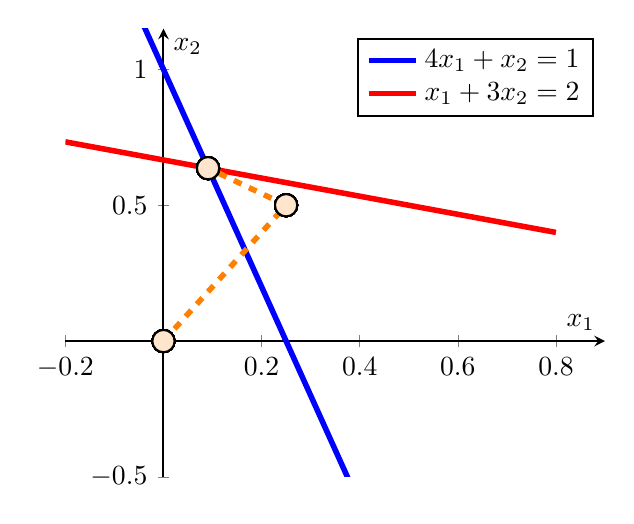
\begin{tikzpicture}
\begin{axis}[axis lines=middle, line width=0.7, enlargelimits=upper, domain=-0.2:0.8, ymin=-0.5, ymax=1, xlabel=$x_1$, ylabel=$x_2$, legend entries={{$4x_1+x_2=1$}, {$x_1+3x_2=2$}}]
\addplot [smooth, color=blue, line width = 2] {1-4*x};
\addplot [smooth, color=red, line width = 2] {(2-x)/3};
\addplot[only marks, mark size=4, color=orange!20, draw=black] (0,0);
\addplot[only marks, mark size=4, color=orange!20, draw=black] (0.25,0.5);
\addplot[only marks, mark size=4, color=orange!20, draw=black] (0.09090909,0.63636364);
\addplot[color=orange, dashed, line width = 2] coordinates {(0,0) (0.25,0.5) (0.09090909,0.63636364)};
\end{axis}
\end{tikzpicture}

\end{document}
